\documentclass[12pt]{article}
\usepackage{graphicx}
\usepackage{fullpage}

\title{Writeup - Numerical Integration}
\author{Lev Teytelman}
\date{\today}

\begin{document}\maketitle
\section{Introduction}

This assignment presented a number of challenges unseen at first. The difficulty came not from the main calculating functions, but from the improvements to be made upon them and the \verb|integrate.c| file.
\section{Scalability and Error Handling}

The functions were not scalable at the start, nor could they handle errors. For example, the \verb|Sqrt| function would not work properly for numbers less than 0. I used an early return to eliminate inputs less than 0, ensuring it would only be calculating the square root of numbers that actually had a square root. The square root function was also extremely slow for large values, which is why I added this code to factor out all twos before calculating the converging series: \begin{verbatim}
    long factoredOut = 1;
    while (x > 1) {
        x /= 4;
        factoredOut *= 2;
    }
\end{verbatim}
This allowed the function to calculate the square root of massive numbers simply by reducing them to small ones, then multiplying by \verb|factoredOut| when returning: \verb|return y * factoredOut;|.

A similar set of checks and processes was added to the Log function: returning if \verb|x| was less than or equal to 0 and dividing by $e$ until \verb|x| was within $[1, e)$: \begin{verbatim}
    if (x <= 0) {
        return x < 0 ? NAN : -INFINITY;
    }
    
    ...
    
    long factoredOut = 0;
    double e = Exp(1);
    while (x > e) {
        x /= e;
        factoredOut++;
    }
\end{verbatim}
The Sin and Cos functions saw a similar improvement, though this time in a method: \begin{verbatim}
double normalize(double x, double interval) {
    return x - (int) (x / interval) * interval;
}
\end{verbatim}
Since sine and cosine waves repeat every $2\pi$, it's enough to normalize them to a low value so the converging series can work with smaller values: \verb|x = normalize(x, 2 * M_PI);|.

The \verb|g| function had the issue of division by zero when $x = 0$. However, the function did not approach any infinity; instead, it approached 1. Therefore, I added a special check in the \verb|functions.c| file: \verb|return x != 0.0 ? Sin(x) / x : 1;|, ensuring there would be no division by 0.

\section{Impact of Partition Amount}

As the number of partitions passed into the \verb|integrate| function increased, the calculated value got closer and closer to the actual one. This makes sense: the smaller and more frequent the rectangles under the graph are, the more accurately they will represent the area.

The trend is apparent with these graphs, with the x label showing the number of partitions passed into the function and the y label being the calculated value:
\begin{figure}\begin{centering}
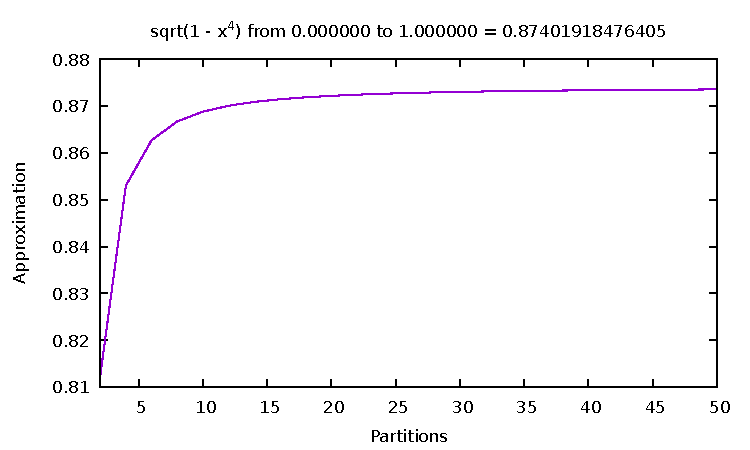
\includegraphics{integrate0.pdf}\caption{The increasing value of $\sqrt{1 - x^4}$ as the number of partitions increases}
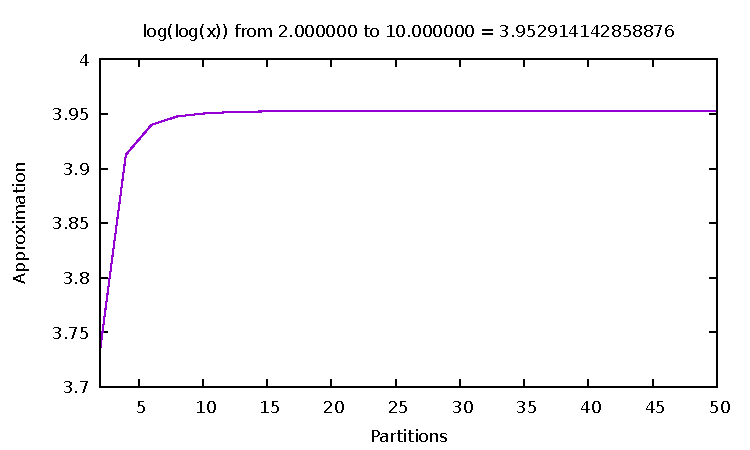
\includegraphics{integrate5.pdf}\caption{The increasing value of $\log{\log{x}}$ as the number of partitions increases}
\end{centering}\end{figure}
\newpage
Notice that the value increases as the partitions get smaller; this is because the original functions' slopes are consistently decreasing, and therefore the large intervals underestimate the value.

Conversely, functions with a mostly increasing slope see an overestimate in their values:
\begin{figure}\begin{centering}
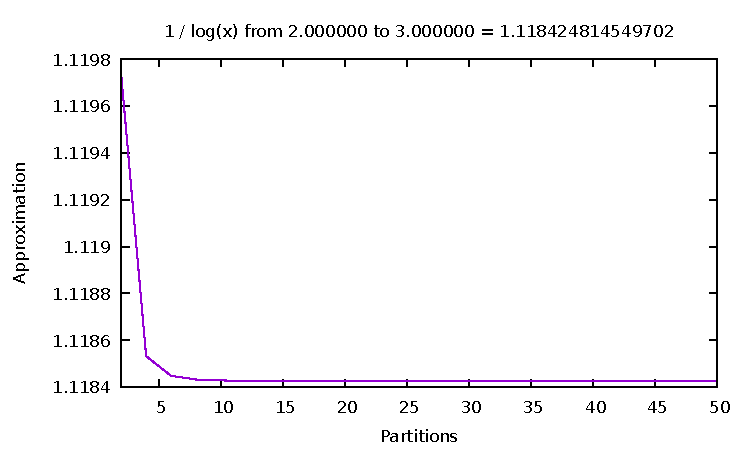
\includegraphics{integrate1.pdf}\caption{The decreasing value of $1 / \log{x}$ as the number of partitions increases}
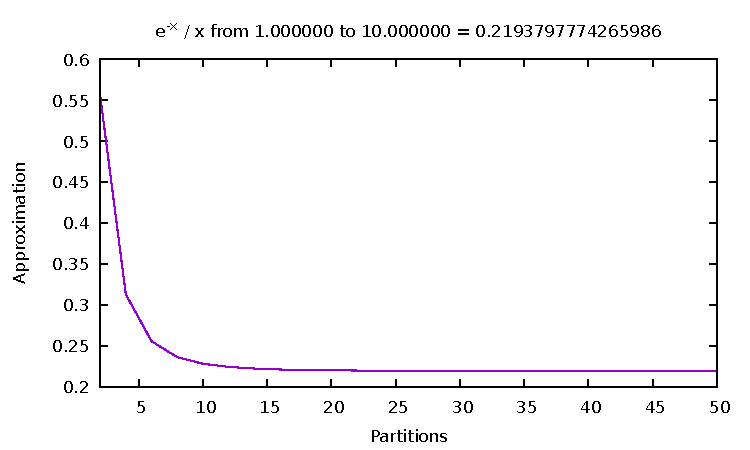
\includegraphics{integrate7.pdf}\caption{The decreasing value of $e^{-x}/x$ as the number of partitions increases}
\end{centering}\end{figure}
\newpage
\begin{figure}\begin{centering}
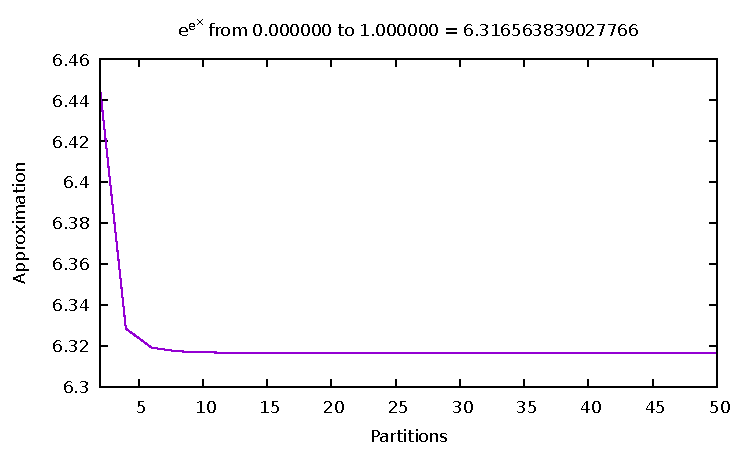
\includegraphics{integrate8.pdf}\caption{The decreasing value of $e^{e^x}$ as the number of partitions increases}
\end{centering}\end{figure}

These estimated values all decrease over time because the function they are calculating the integral of is mostly increasing slope, so the partitions overestimate the area.

Some more interesting graphs are the ones in which the slope is both increasing and decreasing at certain points in time:
\begin{figure}\begin{centering}
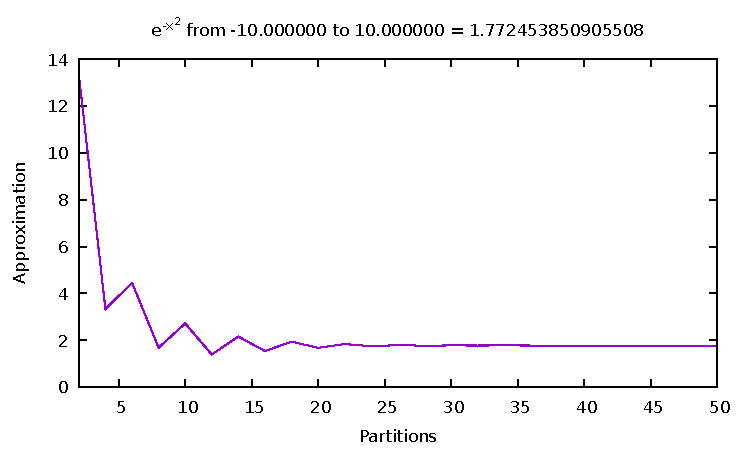
\includegraphics{integrate2.pdf}\caption{The wobbly value of $e^{-x^2}$ as the number of partitions increases}
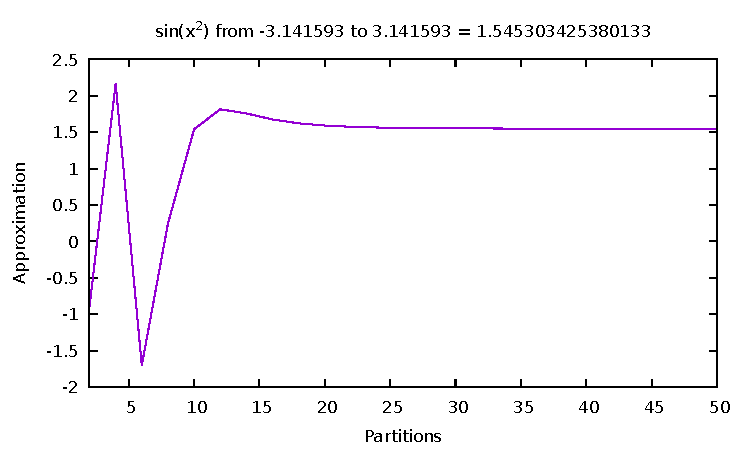
\includegraphics{integrate3.pdf}\caption{The variable value of $sin(x^2)$ as the number of partitions increases}
\end{centering}\end{figure}
\newpage
\begin{figure}\begin{centering}
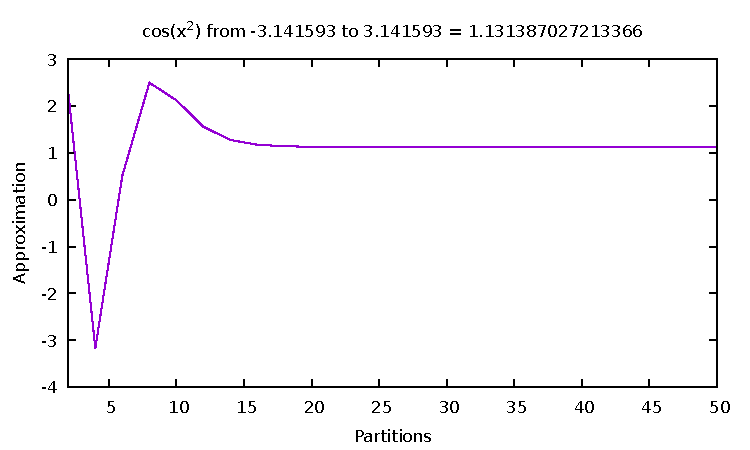
\includegraphics{integrate4.pdf}\caption{The variable value of $cos(x^2)$ as the number of partitions increases}
\end{centering}\end{figure}
Here, the slope changes are mixed between increasing and decreasing, so the estimates fluctuate as they get more precise.

\section{Conclusion}

Overall, the slope change of the underlying function affects the accuracy of early stages of the integral calculations. Functions with positively-increasing slopes (over the given interval) tend to be overestimated by the integration function, while decreasing-slope functions are underestimated. Modifying the program to become more resilient proved interesting: taking the load off of the integration functions and accounting for errors brought out an important, yet often forgotten-about, aspect of programming: modularity and reusability. Luckily, the mathematical functions presented here are resilient and reusable.

\end{document}
